%Disposition
%Affektiv
%pyskotisk
%somatisk

\section{Affektive Lidelser}\label{sec:affektivelidelser}
Denne sektion er primært baseret på \citet{misc:affektivelidelser, misc:netpsykdepression, misc:netpsykmani}.
Affektive lidelser omfatter en række sygdomme hvor stemningslejet afviger fra det habituelle.
Kendetegnende ved sindslidelserne er at de er hyppige og forekommer periodisk.
Dette varierer dog meget, nogle har enkeltstående hændelser mens andre har tilbagevendende episoder.
Der er en stor dødelighed blandt patienter med sygdommen, hovedsagligt grundet selvmord.

Stemningslejet kan afvige fra det habituelle på forskellig vis.
Man skelner mellem mani og depression, hvor unipolare patienter lider af depression, mens bipolare patienter har lidt af minimum en mani periode, med evt. depressions forekomster. Derudover findes der en blandingstilstand hvor man både har depressive og maniske symptomer på samme tid.

Ved depression er stemningslejet sænket, mens det ved mani er løftet.

Der findes forskellige årsager til affektive lidelser. 
Disse inkluderer miljømæssige og arvemæssige forhold, især ved bipolare patienter.
Det skal forstås således at de miljømæssige og arvemæssige forhold gør patienten mere sårbar overfor de affektive lidelser.

Derudover kan somatiske sygdomme såsom blodprop, hjerneblødning og parkinson forårsage mani og depression.
Derudover kan misbrug samt bestemte former for medicin brug forårsage mani og depression.

\subsection{Depression}
Risikoen for at udvikle en depression for kvinder er på ca. 8\% mens den for mænd er på ca. 4\% \citep{misc:affektivelidelser}.
Debutalderen er almindeligvis 40-50 år \citep{misc:affektivelidelser}.
En ubehandlet sygdom varer almindeligvis seks til tolv måneder.
Kroniske depressioner med op til flere års varighed er ikke ualmindelige, især hos ældre \citep{misc:affektivelidelser}.
Derudover er det ca. 15\% af patienterne der kun har en enkeltstående hændelse af depression, hvilket understreger at sygdommen ofte er tilbagevendende.

\citet{misc:netpsykdepression} klassificerer en depression enkeltperiode udfra en række kriterier, der nævnes herefter.
\subsubsection{Depression kriterier}
Følgende information er kopieret fra \citet{misc:netpsykdepression}.

For at opfylde kriterierne for at have en depressiv enkeltepisode i lettere grad skal man:
\begin{itemize}
	\item Have haft depressionen i mere end 2 uger
	\item Ikke tidligere have haft en mani eller en let mani, en såkaldt hypomani
	\item Ikke have en fysisk lidelse som kan forklare symptomerne
\end{itemize}
Man skal have mindst 2 af følgende kernesymptomer:
\begin{itemize}
	\item Man er i dårligt humør og er nedtrykt og trist
	\item Man har nedsat lyst til at foretage sig noget, og man har mere eller mindre mistet interessen for ting, man plejer at interessere sig for
	\item Man bliver hurtigt træt og har ikke så meget energi som man plejer
\end{itemize}
Desuden skal man have mindst 2 af følgende ledsagesymptomer:
\begin{itemize}
	\item Man har nedsat selvtillid eller selvværdsfølelse
	\item Man lider af skyldfølelse og bebrejder sig selv urimeligt
	\item Man har tanker om at det ville være bedre, hvis man var død, eller man tænker på at begå selvmord
	\item Man har svært ved at koncentrere sig eller oplever at man ikke kan tænke klart
	\item Man er enten urolig og hvileløs, eller også er ens bevægelser nærmest gået i stå
	\item Man sover enten mere eller mindre, end man plejer
	\item Man har mistet appetitten og har tabt sig, eller man er begyndt at trøstespise og har taget på
\end{itemize}

\subsubsection{Grader af depression}
Man skelner mellem forskellige grader af depression.
Depression i lettere grad vil sige at man er i stand til at bibeholde sine sædvanlige aktiviteter selvom man har det dårligt.
Ved depression i moderat grad har man svært ved at forsætte med sin sædvanlige aktiviteter grundet hvor dårligt man har det, derudover har man fire ledsagesymptomer og ikke kun tre
Har man en svær depression kan man ikke fortsætte med sine normale aktiviteter, derudover har man alle tre kernesymptomer og fem ledsagesymptomer.

\subsubsection{Individuelle Symptomer}
Det er vigtigt for patienter der lider af depression at de er opmærksomme på hvad der er symptomer for at en depression er på vej for dem.
Dette afhænger meget af individet, men starter ofte på samme måde som tidligere for det enkelte individ.
Eksempler på dette kan være en overfladisk søvn, vågner tidligt, bekymringer om bagateller etc.
Det kan også være at patienten bliver dvask og sover længe.

Hvis disse symptomer opfanges kan behandling af depressionen påbegyndes tidligere i forløbet og i bedste tilfælde forhindres.
\subsubsection{Selvbehandling}
Man kan nedsætte risikoen for en depression hvis man har en sund livsstil.
Dette inkluderer at spise sundt mad, at dyrke motion og undgå at indtage rusmidler.
Desuden informerede kontaktpersonen \citet{misc:janne-rasmussen} at til behandling af depression opfordres patienten til at foretage en mængde af lystbetonede aktiviteter.

\subsection{Mani}
Risikoen for at udvikle en mani, og derved en bipolar sygdom, er ca. 1-2\%, og er således lige hyppig blandt mænd og kvinder.
Dog er det ofte at sygdommen er tilbagevendende, da der er en risiko på ca. 90\% for at få en ny episode på et senere tidspunkt.
Debutalderen for sygdommen er almindeligvis før 30-års alderen, og ved omkring halvdelen af patienterne forekommer sygdommen før man er 20 år.
Varigheden for sygdommen er i ubehandlede tilfælde typisk mellem to og otte måneder, men der findes her også kroniske tilfælde,

\citet{misc:netpsykmani} klassificerer en manisk enkeltepisode uden psykotiske symptomer som at man i mere end en uge skal opfylde følgende:
\begin{itemize}
	\item Have været opstemt, eksalteret og irritabel.
	\item Hvis man er opstemt eller eksalteret have mindst tre af følgende symptomer. Hvis man især er irritabel skal man op på mindst fire symptomer:
	\begin{itemize}
		\item Man er hyperaktiv, rastløs og urolig
		\item Man føler et indre pres for at tale uafbrudt
		\item Man har tankeflugt, hvor tankerne springer fra emne til emne
		\item Man har en hæmningsløs adfærd, hvor ens normale hæmninger er væk
		\item Man har nedsat behov for søvn
		\item Man har forhøjet selvfølelse, grandiositet
		\item Man er usamlet eller bliver konstant distraheret
		\item Man handler hensynsløst og uansvarligt
		\item Man har større seksualdrift end normalt
	\end{itemize}
	\item Ikke have haft hallucinationer eller vrangforestillinger
	\item Symptomerne må ikke skyldes en fysisk sygdom
\end{itemize}
Hvis man derimod har en mani med psykotiske symptomer svarer den til symptomerne for en manisk enkeltepisode uden psykotiske symptomer, men hvor man har haft hallucinationer, eller vrangforestillinger. Dog ikke bizzare vrangforestillinger såsom ved skizofreni.

Derudover kan man også have hypomani der er en lettere grad for mani, hvor man blot i mere end fire dage skal have en manisk episode.

\subsubsection{Individuelle Symptomer}
Det er individuelt hvilke symptomer de enkelte patienter har på en begyndende mani periode.
Dog starter perioden ofte på samme måde som tidligere perioder.
Eksempelvis kan man være meget aktiv, rastløs, have mindre brug for søvn, ekstatisk etc.

Ligesom depression er det vigtigt at opdage episoderne i de begyndende stadier, da man også her på den måde ville kunne mindske eller helt undgå episoden.
Derudover kan en depression følge efter en mani periode, og man kan derfor også mindske risikoen for disse episoder \citep{misc:bipolarsundhed}.

\subsubsection{Selvbehandling}
Man skal undgå at drikke alkohol når man er i en manisk periode, da det kan forværre perioden \citep{misc:netpsykmani}.
Derudover gælder det om at begrænse mængden af stimuli, og generelt forsøge at tage det mere med ro \citep{misc:janne-rasmussen}.

\subsection{Bipolar lidelse}
En bipolar lidelse er kendetegnende ved minimum en manisk episode og evt. depression episoder.
Et eksempel på dette med en stemningsleje graf over tid kan ses i \figref{fig:stemningslejegrafeksempel}.

\begin{figure}
	\centering
	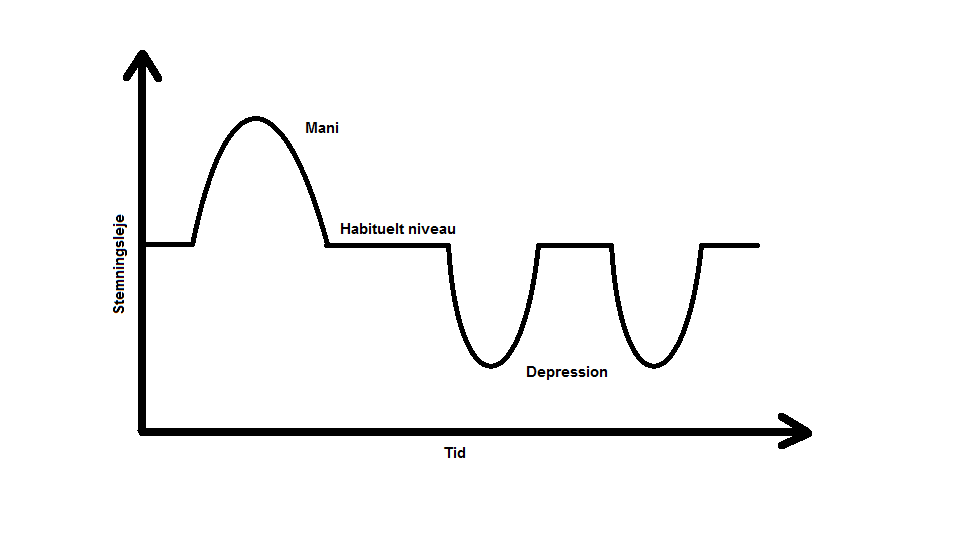
\includegraphics[scale=0.5]{media/affektivstemningsleje}
	\caption{Graf over stemningsleje for en patient med en mani og to depressions perioder.}\label{fig:stemningslejegrafeksempel}
\end{figure}

Det oftest sete er en mani episode og flere depressions episoder, men andre scenarier kan også forekomme.
Det gælder således om at have patienten på det habituelle niveau og hurtigt opdage når en patient afviger fra dette.